
\section{Experiments}
\label{sec:exp}

%\subsection{Settings}

To investigate whether the psychiatrist can improve his diagnostic skills, our core experiments lie on whether an \system~ elevates dialogue quality and depression diagnosis accuracy. The general settings, including training strategy and metrics, are introduced below.


\paragraph{Settings}
Since \system's architecture has a supervisor plugin to conduct reflection, we follow the same experiment setting as previous works~\cite{shinn2023reflexion, renze2024selfreflectionllmagentseffects} in the training stage. The psychiatrist agent generates the diagnosis result through Equation~\ref{eq:vote}.

% \MY{still unclear here, just give clear definitions to how you train, how you evaluate using Quiz and Exam.}
% please paraphrase and rewrite these sentences, there are two settings (or we say splits), first is Quiz, which uses train set. second is Exam, which uses test set . both of the datasets are detailed in \S\ref{}.

The experiments involve two distinct settings: Quiz and Exam, evaluate on either train set or test set detailed in \S\ref{train/test}. In the \textbf{Quiz} setting, the psychiatrist agent works with the \textit{train set}. After each conversation, it generates a diagnosis result. If the result is incorrect, the agent receives feedback from the supervisor to refine its diagnostic skills and attempts the diagnosis again. This process tests the self-refinement capability of the LLMs, allowing the agent to improve its performance over time, even when applied to unseen patients.

In the \textbf{Exam} setting, the psychiatrist agent is evaluated on the \textit{test set}. Here, the agent generates a diagnosis result based on the knowledge and memory it accumulates from the Quiz setting. Unlike the Quiz, the agent only has one opportunity to provide a diagnosis without a second attempt if the initial result is incorrect. This setting is designed to assess the agent's generalization ability, reflecting the real-world scenario where a diagnosis is made without the chance for revision.

% \textbf{Train Split} is the train set selected in \S\ref{train/test}, the psychiatrist agent generates diagnosis result after the conversation. If the result is incorrect, the psychiatrist agent reflects diagnosis skills with the help of the supervisor, and diagnosis once more.
% \textbf{Test Split} is the original test set of D$^4$, defined as the cases only for evaluation, the psychiatrist provides diagnosis result based on all the memory generated on \textbf{Train Split}. The experiments conducted on train split evaluate the self-refine capability of LLMs, where the psychiatrist agent can correct its answer based on the feedback, leading to a better performance, even on \textbf{Test Split}. We describe it as \textbf{Quiz}.
% \textbf{Test Split} is referred as \textbf{Exam}, which are cases for the psychiatrist agent to examine the generalization capability of the psychiatrist agent observing and reflecting on the train set.

% Accordingly, the psychiatrist agent generates the diagnosis result only once, without a second chance if the result is incorrect, which aligns with the diagnosis procedure in real life.

%If the diagnosis aligns with the depression and suicide risks provided by the supervisor plugin, we will record the diagnosis result. 
%Otherwise, the supervisor will stimulate the psychiatrist to summarize skills and perform a second diagnosis, which we will then record. As for the baseline, the psychiatrist will conduct a second diagnosis without reflection if the initial diagnosis is incorrect, ensuring fairness.
We use \texttt{gpt-3.5-turbo-0125} \cite{chatgpt} for the content generation and \texttt{text-embedding-ada-002} to get embeddings of the content.

\paragraph{Metrics} Two accuracy aspects are involved:
depression risk prediction accuracy and suicide risk prediction accuracy, we also report their average score as overall accuracy. For each patient agent, the risk of depression and the risk of suicide are classified into four categories: control, mild, moderate, or severe.
% while the existence of each symptom is divided into unclear, true, or false. 

\paragraph{Results: Does AMC work?}
To extensively validate whether AMC works, we conduct the main experiments under two scenarios:
\begin{enumerate}
    \item \textbf{Original Dialogue (OD)}, \system~takes the original dialogue history in D$^4$ as the conversation between the psychiatrist agent and the patient agent, in order to eliminate the bias of role-playing. The psychiatrist agent conducts the diagnosis directly based on this dialogue. %\MY{This setting can be seen as a topline for dialogue simulation.(?)}
    \item \textbf{Simulated Dialogue (SD)}, \system~generates simulated diagnosis dialogues between the psychiatrist agent and the patient agent, with the psychiatrist agent performing the diagnosis based on this newly generated dialogue. 
\end{enumerate} 

For each scenario, we construct experiments on two settings: 1) Deactivate the memory module of the psychiatrist agent, evaluating the baseline capability of original LLMs, denoted as \textit{w/o} memory. 2) Activate the memory module and retrieve 10 memory nodes from EMR and skills, denoted as \textit{w/} memory. % 10+10 
% In order to fully evaluate the effectiveness of EMR and skills, we 


We present the results in Table~\ref{tab:main}, which demonstrate the efficacy of the memory module and reflection function on almost all settings, with stable improvements. Across original and simulated dialogues, the largest performance gain from memory and reflection is achieved on \textit{depression diagnosis accuracy}, where even in the most difficult setting (test cases in simulated dialogues), an increase of $6.8\%$ is observed. However, the performance of experiments on simulated dialogues has a significant decrease, despite the improvement of memory structure. The experiment result indicates the limited capability of LLMs to describe the symptoms precisely based on patient profiles. We attach the case study in the appendix, which can further explore the role-play ability of LLMs in diagnostic scenarios.
%\MY{ Further, there is still room for improvement since the accuracy discrepancy between original and simulated, train and test is significant. PLEASE add explanation, since the general accuracy is still low.}

%\ZC{explain results here.}

\textit{\textbf{Take Home Message: } Memory module and reflection function significantly enhance depression diagnosis accuracy, especially in challenging scenarios, but LLMs struggle with precisely simulating symptoms in diagnostic dialogues, highlighting role-play limitations.}


\paragraph{Effects of different memories}

To investigate the impact of different memory types on depression diagnosis, we conduct an experiment by manipulating the activation levels of memories: 1) Deactivating the memory module, 2) Activating the memory module and retrieving memories from electronic medical records (EMR), 3) Retrieving memories based on diagnostic skills, and 4) Retrieving memories from both EMR and diagnostic skills. The results of the experiment are depicted in Figure~\ref{fig:exp}. 

From the bar charts, it is evident that in OD settings, diagnostic skills are more effective, likely due to their role in aligning LLMs. Additionally, EMR appears to be more beneficial when dialogues are simulated (SD). This is because the simulated dialogues lack the precision of original diagnosis dialogues, and EMR can assist the psychiatrist agent by retrieving similar patient cases for a more accurate diagnosis. Furthermore, the results show that leveraging both EMR and diagnostic skills yields better and more stable performance than relying on the original LLMs alone.


\begin{figure}[!t]
    \centering
    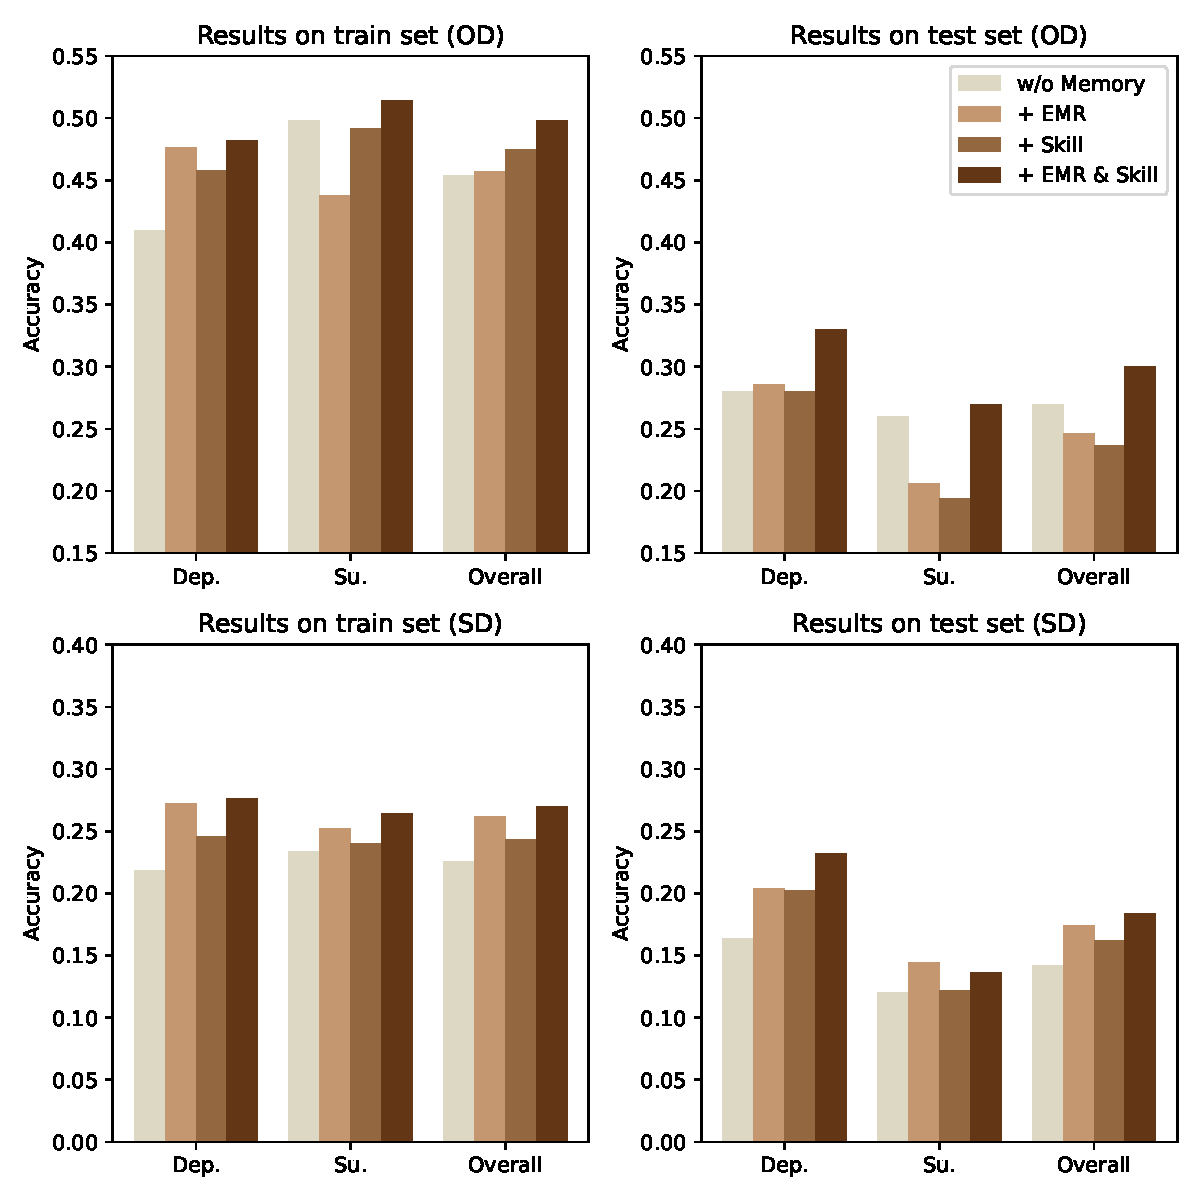
\includegraphics[width=1\linewidth]{fig/experiments_memory_new.pdf}
    \caption{\textbf{The Results of Ablation Study on Memory Layers.} The first row indicates the results based on the original dialogue history setting, while the second row implies the results based on the simulated dialogue setting. At the same time, the first column suggests the results on the train set, while the second column indicates the results of the test.}
    \label{fig:exp}
\end{figure}

\textit{\textbf{Take Home Message: } Combining multi-level memory enhances depression diagnosis, ensuring stable and improved performance across settings.}


\paragraph{Effects of supervisor plugin}


To validate the function of the supervisor plugin, we conduct an ablation experiment by disabling the guidance reflection and generation features. The results are presented in Table~\ref{tab:plugin}. The experiment demonstrated that the supervisor plugin improves the accuracy of risk prediction. 
% However, we also observe an interesting phenomenon: while the supervisor plugin enhances the accuracy of depression and suicide predictions, it slightly decreases the accuracy of symptom prediction.
% This outcome can be explained by the design of the supervisor plugin, which explicitly guides the system to focus on one aspect of inquiry per round. This focused approach leads to a more in-depth exploration of fewer topics, thereby improving the accuracy of predictions for depression and suicide risks. On the other hand, when the guidance is disabled, the system tends to inquire about multiple symptoms within a single turn, allowing it to gather threads of information at one time. This broader approach can result in more accurate symptom screening within the limited number of interaction rounds.

\textit{\textbf{Take Home Message: } The supervisor plugin enhances targeted risk predictions.}
 % but may reduce symptom screening accuracy due to focused inquiry



% To validate the function of the supervisor plugin, we conducted an ablation experiment by disabling the guidance reflection and generation. The results are listed in Table~\ref{tab:plugin}. The experiment result demonstrated that the supervisor plugin can

%\MY{Interestingly, supervisor provides accuracy improvement on depression and suicide prediction however decreases symptom accuracy. PLEASE provide explaination here!}

% 由于我们在supervisor plugin里面明确要求由其引导psy 进行提问,而每一轮的问诊限制在一个方面,因而在有限轮数的问诊中,医生倾向于基于较少的话题进行较为深入的询问,which 解释了depresson和suicide risk准确率的提升;而在无指导的情况下,则医生可能会选择在一次对话中询问多个症状,因而能够在有限轮数中获取更加完整的信息,获得更好的症状筛选准确率。

\begin{table}[htbp]
    \centering
    \small
    \setlength{\tabcolsep}{3pt}
    \begin{tabular}{ccccc}
        \toprule
        \textbf{Setting} & \textbf{Plugin} & Dep. & Su.  & \textbf{Overall} \\
        \midrule
        \multirow{2}{*}{\makecell[c]{\textbf{Quiz}\\(Train)}} & w/o & 24.0   & 25.2  &    \cellcolor{gray!30}  24.6   \\
                                        & w/  & 27.6(+3.6)  & 26.4(+1.2) & \cellcolor{gray!30} 27.0 (+2.4)       \\
        \midrule
        \multirow{2}{*}{\makecell[c]{\textbf{Exam}\\(Test)}}  & w/o &  22.0  & 12.0 & \cellcolor{gray!30}17.0      \\
                                        & w/  & 23.2(+1.2) &  13.6(+1.6)    &  \cellcolor{gray!30}18.4(+1.4)          \\
        \bottomrule
    \end{tabular}
    \caption{\textbf{Effects of Supervisor Plugin in Reflection and Providing Feedback.}}
    % (Ref): enable reflection if the prediction of the first attempt is incorrect, this is not adopted in the test set.
    \label{tab:plugin}
\end{table}

%\KZ{Stuff is missing here!}






% \subsection{Ablation study on further diagnosis\ZC{second-time diagnosis to see if the doctor could give more accurate results}} 

% \textit{\textbf{Take Home Message: } This is a take home message.}

% \begin{table}[htbp]
%     \centering
%     \small
%     \setlength{\tabcolsep}{3pt}
%     \begin{tabular}{cccccc}
%         \toprule
%         \textbf{Dataset} & \textbf{Setting} & Dep. & Su. & Sym. & \textbf{Overall} \\
%         \midrule
%         \multirow{4}{*}{\textbf{OD}} & w/o &      &   &    &    \cellcolor{gray!30}     \\
%                                         & w/  & 26.2(+)  & 24.4(+)  & 36.8(+)  & \cellcolor{gray!30}87.4(+)       \\
%         \midrule
%         \multirow{4}{*}{\textbf{SD}}  & w/o &  22.0  & 12.0  & 36.2 & \cellcolor{gray!30}23.4      \\
%                                         & w/  & 21.0(-1.0) &  13.6(+1.6)  & 34.2(-2.0)    &  \cellcolor{gray!30}22.9(-0.5)          \\
%         \bottomrule
%     \end{tabular}
%     \caption{\textbf{The main experiment results on depression diagnosis.} Dep. Acc.: the accuracy of depression risk classification. Su. Acc.: the accuracy of suicide risk classification. Sym. Acc.: the average accuracy of symptom prediction. EMR: electronic medical records concluded by the reflection module. Skill: the summarized skill reflected by the reflection module. }
%     % (Ref): enable reflection if the prediction of the first attempt is incorrect, this is not adopted in the test set.
%     \label{tab:exp}
% \end{table}



%\MY{We need a paragraph to say how many different experiments are done, and how they differ from each other.i.e. To investigate the efficacy of AMC, we test the depression diagnosis, suicide risk prediction, and symptom accuracy under 4 different settings (which from easy to hard xxxxx). can you list them in short and we can discuss later tonight?}


% \subsection{Risk Classification with D$^4$ History}
% In risk classification experiments with D$^4$ history, the experiment result can be shown in the first row of Figure \ref{fig:exp}. From the result, we can figure out that electronic medical records and summarized skills can both improve the performance of the depression diagnosis, while summarized skills might be more useful since they provide direction for alignment. The results demonstrate the effectiveness of reflection module and memory module on current patient case. 

% However, we need extra experiment to evaluate the effectiveness of memory generated from different patient cases. Therefore, we conduct the experiments based on the psychiatrist agent storing the memory generated based on the train set, which labeled as \textbf{Train(Exp)}. In the meanwhile, previous works mainly focus on trial and error possible tasks such as code generation, so these works can conduct reflection during test stage. However, our simulation based on diagnosis is not a trial and error possible task. Taking these considerations into account, we deactivate reflection module except the training stage, which means we will not diagnosis once more if the psychiatrist agents provide a incorrect diagnosis result.

% The experiment result of \textbf{Train(Exp)} is presented in the second block of Table~\ref{fig:exp}. The experiment also shows the improvement of **.

% After showing the effectiveness of reflection module in train set in with experience and without experience settings, we utilized testset D$^4$ utilized to demonstrate the helpfulness of generated memory nodes on unseen cases. The experiment result is presented in the third block of Table~\ref{tab:complete}. The experiment result demonstrated generated skills are useful for aligning the LLMs to the risk distribution in real-life scenarios.

% After demonstrating the effectiveness of tertiary memory structure and sampling memory module on diagnosis dialogue in real life, we tested whether the architecture can be useful in simulated conversation generation scenarios. In the experiment, depression diagnosis results are generated after a conversation between the psychiatrist agent and potential patient agents. The experiment result can be shown as Table~\ref{tab:complete}. From the experiment result, we can figure out that the reflection module is effective even in simulated diagnosis procedures.

% \subsection{Risk Classification with Simulated Dialogues}

% To eliminate the effects of Role-playing bias during diagnosis conversation to demonstrate the effects of reflection modules, we first utilized normal depression risk classification setting on the psychiatrist agent without reflection module, which takes the original dialogue history from D$^4$ as input, while outputs the depression risk classification, suicide risk classification and the predicted detailed symptoms list. After conducting the original risk classification experiment, we activate the memory module and reflection module, then conduct the same experiment with different settings: whether we provide the electronic medical record, summarized skills or both. 
